%%
%% Automatically generated file from DocOnce source
%% (https://github.com/hplgit/doconce/)
%%
%%


%-------------------- begin preamble ----------------------

\documentclass[%
oneside,                 % oneside: electronic viewing, twoside: printing
final,                   % draft: marks overfull hboxes, figures with paths
10pt]{article}

\listfiles               %  print all files needed to compile this document

\usepackage{relsize,makeidx,color,setspace,amsmath,amsfonts,amssymb}
\usepackage[table]{xcolor}
\usepackage{bm,ltablex,microtype}

\usepackage[pdftex]{graphicx}

\usepackage[T1]{fontenc}
%\usepackage[latin1]{inputenc}
\usepackage{ucs}
\usepackage[utf8x]{inputenc}

\usepackage{lmodern}         % Latin Modern fonts derived from Computer Modern

% Hyperlinks in PDF:
\definecolor{linkcolor}{rgb}{0,0,0.4}
\usepackage{hyperref}
\hypersetup{
    breaklinks=true,
    colorlinks=true,
    linkcolor=linkcolor,
    urlcolor=linkcolor,
    citecolor=black,
    filecolor=black,
    %filecolor=blue,
    pdfmenubar=true,
    pdftoolbar=true,
    bookmarksdepth=3   % Uncomment (and tweak) for PDF bookmarks with more levels than the TOC
    }
%\hyperbaseurl{}   % hyperlinks are relative to this root

\setcounter{tocdepth}{2}  % levels in table of contents

% Tricks for having figures close to where they are defined:
% 1. define less restrictive rules for where to put figures
\setcounter{topnumber}{2}
\setcounter{bottomnumber}{2}
\setcounter{totalnumber}{4}
\renewcommand{\topfraction}{0.95}
\renewcommand{\bottomfraction}{0.95}
\renewcommand{\textfraction}{0}
\renewcommand{\floatpagefraction}{0.75}
% floatpagefraction must always be less than topfraction!
% 2. ensure all figures are flushed before next section
\usepackage[section]{placeins}
% 3. enable begin{figure}[H] (often leads to ugly pagebreaks)
%\usepackage{float}\restylefloat{figure}

% prevent orhpans and widows
\clubpenalty = 10000
\widowpenalty = 10000

% --- end of standard preamble for documents ---


% insert custom LaTeX commands...

\raggedbottom
\makeindex
\usepackage[totoc]{idxlayout}   % for index in the toc
\usepackage[nottoc]{tocbibind}  % for references/bibliography in the toc

%-------------------- end preamble ----------------------

\begin{document}

% matching end for #ifdef PREAMBLE

\newcommand{\exercisesection}[1]{\subsection*{#1}}


% ------------------- main content ----------------------



% ----------------- title -------------------------

\thispagestyle{empty}

\begin{center}
{\LARGE\bf
\begin{spacing}{1.25}
Theory for Exploring Nuclear Structure Experiments
\end{spacing}
}
\end{center}

% ----------------- author(s) -------------------------

\begin{center}
{\bf Nuclear TALENT COURSE 2017}
\end{center}

    \begin{center}
% List of all institutions:
\centerline{{\small The European Center for Theoretical Nuclear Physics and Related Areas, Trento, Italy}}
\end{center}
    
% ----------------- end author(s) -------------------------

% --- begin date ---
\begin{center}
July 3-21, 2017
\end{center}
% --- end date ---

\vspace{1cm}


\subsection*{TALENT course 2017}

Applications are open for the 2017 TALENT course on 
\textbf{Theory for exploring Nuclear Structure experiments}.  The recently established
initiative, Nuclear TALENT (Training in Advanced Low Energy Nuclear Theory), 
see also \href{{http://www.nucleartalent.org}}{\nolinkurl{http://www.nucleartalent.org}}, a multi-national network of
several European and North American institutions, aims to develop a
broad curriculum that will serve as a platform for cutting-edge theory
of nuclei and their reactions.


This year the Nuclear TALENT initiative organizes a course on 
"Theory for Exploring Nuclear Structure Experiments" to be held at
at The European Center for Theoretical Nuclear Physics and Related Areas
(ECT*), Trento, Italy from July 3 to July 21 2017. 

\subsection*{Lecturers}
The lecturers are 
\begin{enumerate}
\item \href{{https://people.nscl.msu.edu/~brown/}}{Alex Brown}, \href{{http://www.nscl.msu.edu/}}{National Superconducting Cyclotron Laboratory} and \href{{https://www.pa.msu.edu/}}{Department of Physics and Astronomy}, \href{{http://www.msu.edu/}}{Michigan State University}, East Lansing, MI 48824, USA

\item \href{{https://people.nscl.msu.edu/~gade/}}{Alexandra Gade}  \href{{http://www.nscl.msu.edu/}}{National Superconducting Cyclotron Laboratory} and \href{{https://www.pa.msu.edu/}}{Department of Physics and Astronomy}, \href{{http://www.msu.edu/}}{Michigan State University}, East Lansing, MI 48824, USA

\item \href{{http://web.utk.edu/~rgrzywac/}}{Robert Grzywacz}  at \href{{http://www.ornl.gov/}}{Oak Ridge National Laboratory}, Oak Ridge, TN 37831  and \href{{https://www.phys.utk.edu/}}{Department of Physics and Astronomy}, \href{{http://www.utk.edu/}}{University of Tennessee}, Knoxville, TN 37996-1200, USA

\item \href{{http://mhjgit.github.io/info/doc/web/}}{Morten Hjorth-Jensen}  at \href{{http://www.nscl.msu.edu/}}{National Superconducting Cyclotron Laboratory} and \href{{https://www.pa.msu.edu/}}{Department of Physics and Astronomy}, \href{{http://www.msu.edu/}}{Michigan State University}, East Lansing, MI 48824, USA and  Department of Physics, University of Oslo, N-0316 Oslo, Norway

\item \href{{https://www.ornl.gov/staff-profile/gustav-r-jansen}}{Gustav Jansen}  at \href{{http://www.ornl.gov/}}{Oak Ridge National Laboratory}, Oak Ridge, TN 37831, USA
\end{enumerate}

\noindent
\subsection*{How to apply and teaching material}

\textbf{The deadline for applications is April 15, 2017}.  
For more information on how  to apply see \href{{http://ectstar.eu/node/797}}{\nolinkurl{http://ectstar.eu/node/797}},
see also \href{{http://ectstar.eu/node/2240}}{\nolinkurl{http://ectstar.eu/node/2240}}. A detailed content list can be found at
\href{{http://nucleartalent.github.io/NuclearStructure/doc/web/course.html}}{\nolinkurl{http://nucleartalent.github.io/NuclearStructure/doc/web/course.html}}.

The target groups are Master of Science and PhD students and
early post-doctoral researchers, both experimentalists and
theorists interested in models for nuclear
structure, phenomenological techniques for interpreting and predicting
the structure of stable as well as exotic nuclei. More experienced researchers may apply, but will be
considered only on a fully-self-supported basis if numbers and space
permit. Local support is available for at most 15-20 participants.



\subsection*{Organizers}

\begin{enumerate}
\item \href{{https://people.nscl.msu.edu/~brown/}}{Alex Brown}, \href{{http://www.nscl.msu.edu/}}{National Superconducting Cyclotron Laboratory} and \href{{https://www.pa.msu.edu/}}{Department of Physics and Astronomy}, \href{{http://www.msu.edu/}}{Michigan State University}, East Lansing, MI 48824, USA

\item \href{{http://mhjgit.github.io/info/doc/web/}}{Morten Hjorth-Jensen}, \href{{http://www.nscl.msu.edu/}}{National Superconducting Cyclotron Laboratory} and \href{{https://www.pa.msu.edu/}}{Department of Physics and Astronomy}, \href{{http://www.msu.edu/}}{Michigan State University}, East Lansing, MI 48824, USA and Department of Physics, University of Oslo, N-0316 Oslo, Norway 
\end{enumerate}

\noindent
Morten Hjorth-Jensen will also function as student advisor and coordinator.

\subsection*{Additional information}

For additional information on each of the courses, please see
\href{{http://www.nucleartalent.org}}{\nolinkurl{http://www.nucleartalent.org}}. Prior to the TALENT course, the ECT* organizes 
a Doctoral Training program on Microscopic Theories of Nuclear Structure, Dynamics and 
Electroweak Currents from June 12 to June 30, 2017. 
The doctoral training program can be combined with the TALENT course.
Applicants interested in attending the doctoral training program can find more information at
\href{{http://ectstar.eu/node/2238}}{\nolinkurl{http://ectstar.eu/node/2238}}.





\vspace{6mm}

% inline figure
\centerline{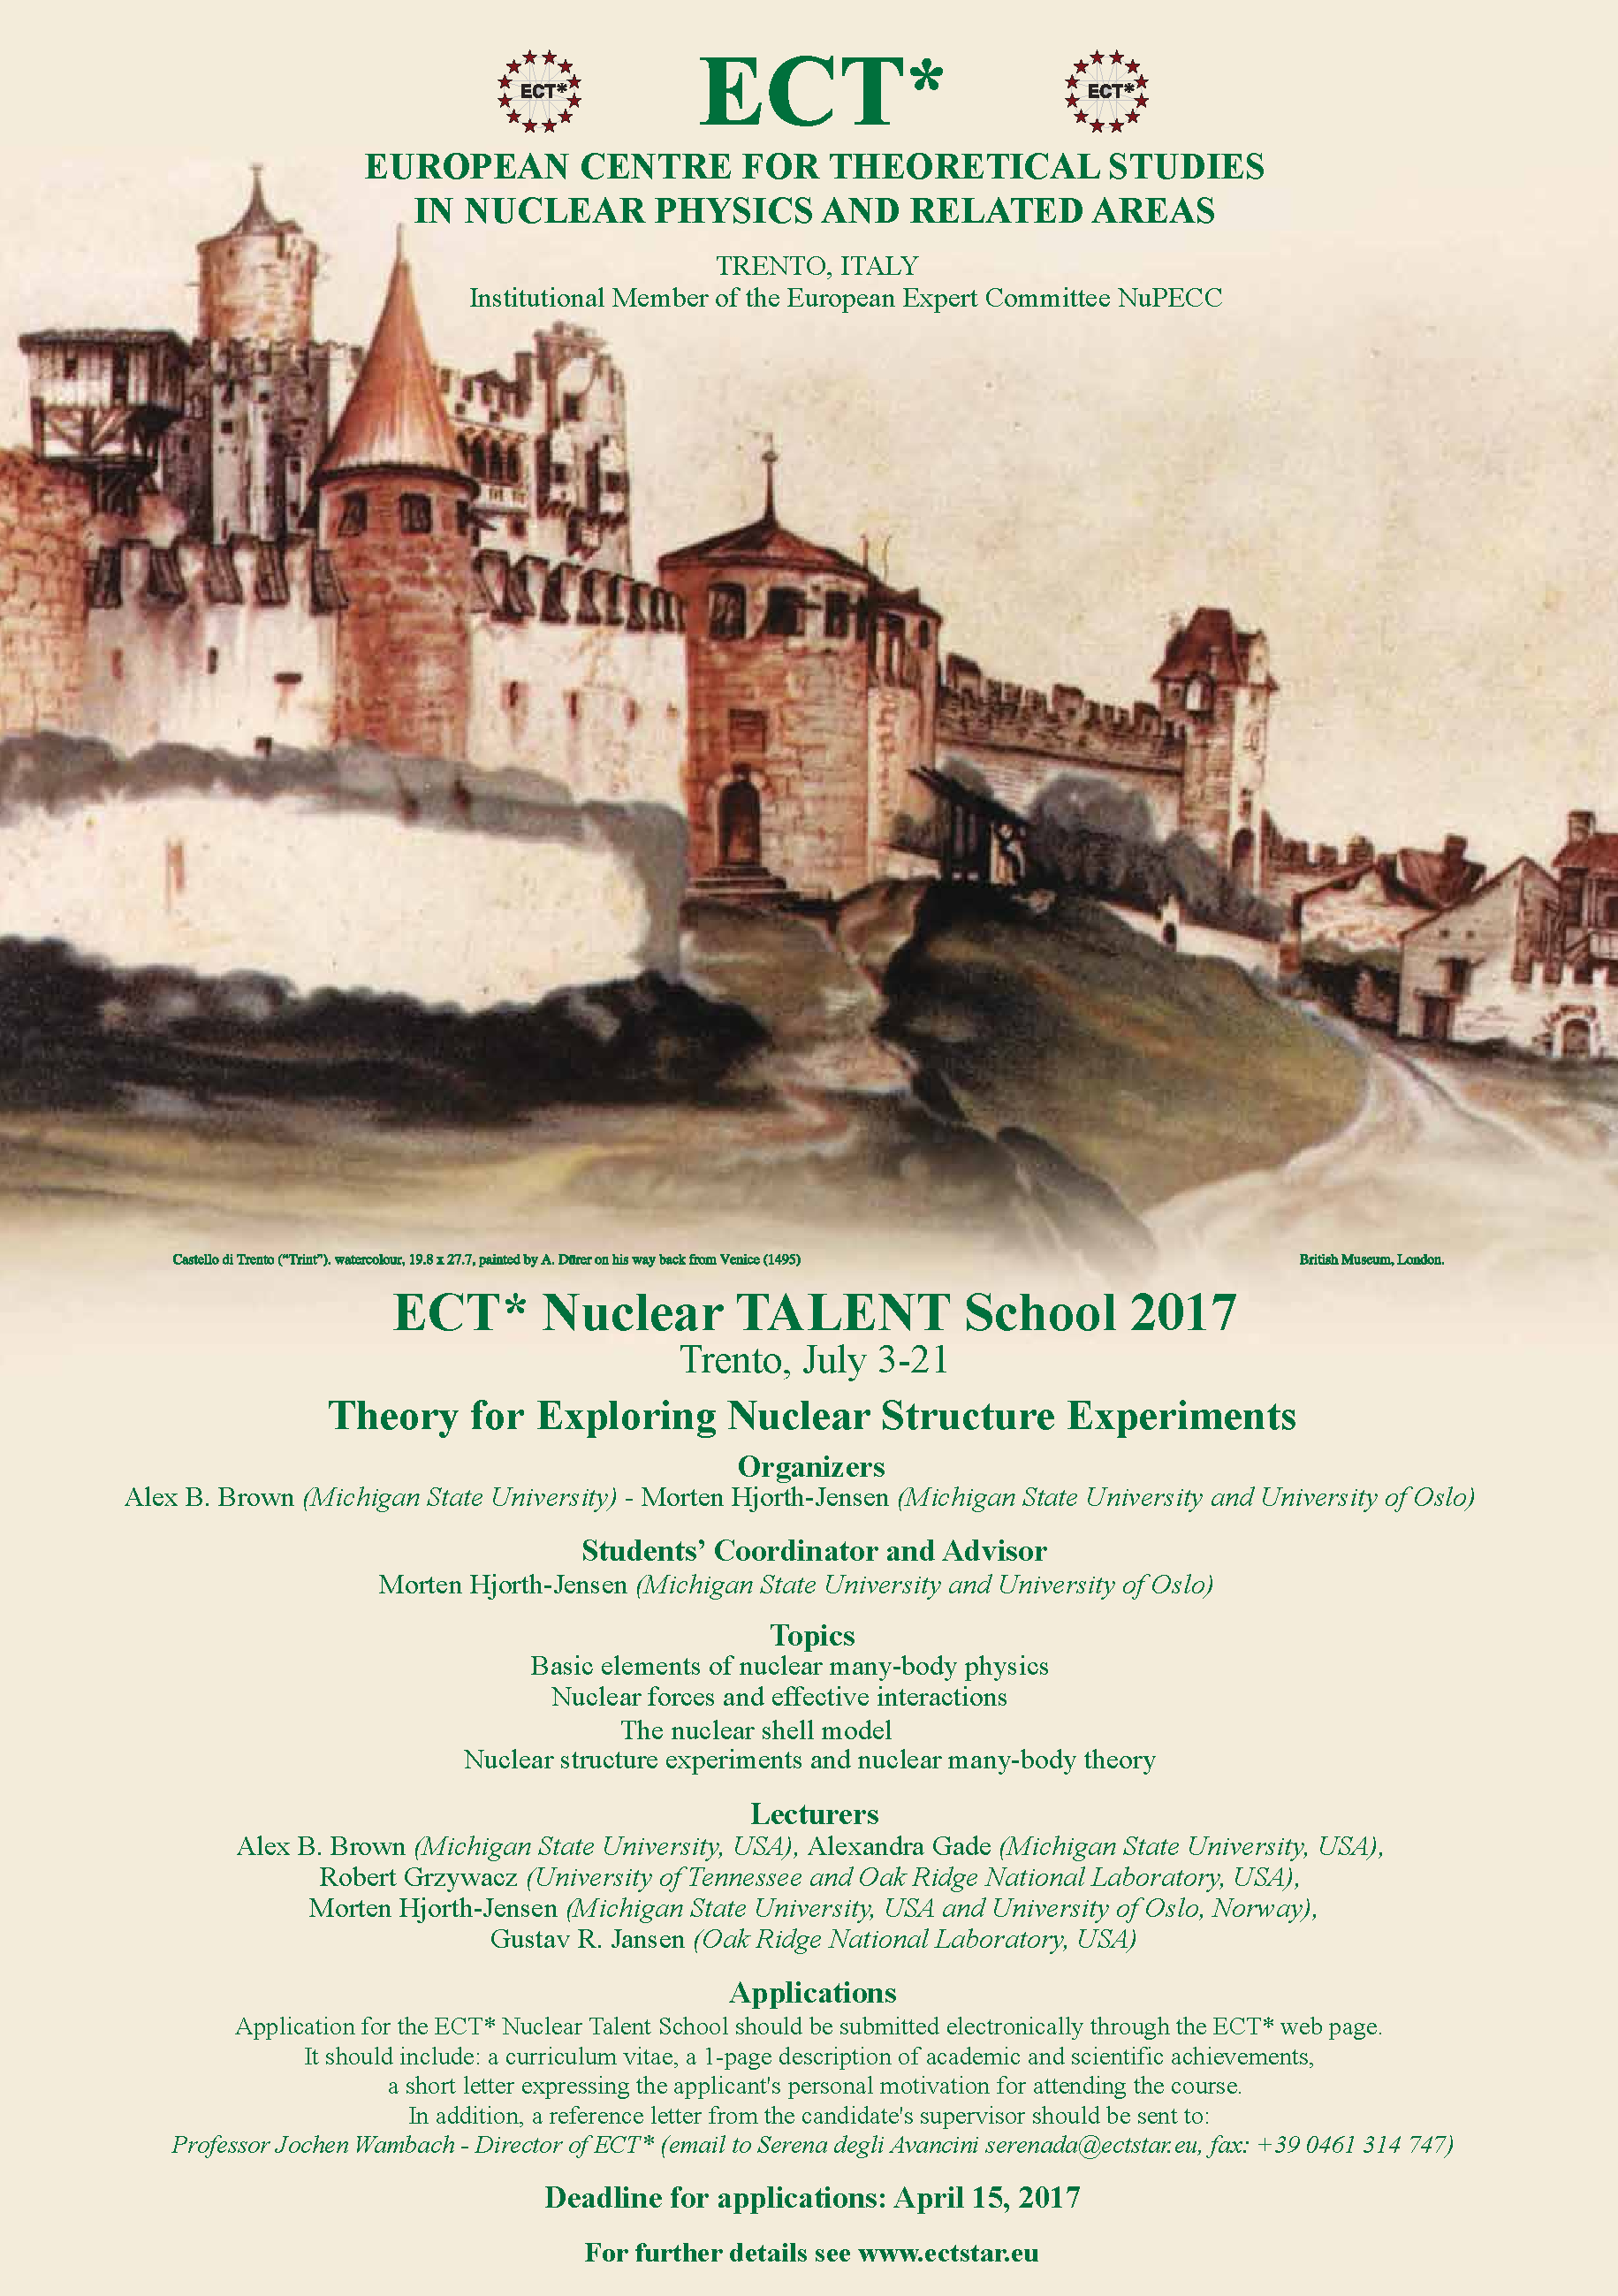
\includegraphics[width=1.0\linewidth]{Poster.pdf}}

\vspace{6mm}




% ------------------- end of main content ---------------

\end{document}

